\subsection{Experiment 9: Regularization Techniques and Training Progress for Rebuilt Model} \label{sec:exp9}

In this study, the author employed regularization techniques while holding all other parameters constant to build upon the previous experiment.

Nonetheless, an unforeseen crash transpired at epoch 34, resulting in a substantial reduction in loss values that ultimately converged to zero. It is crucial to note that all presented values are objective and exclusively quantitative.

The experiment incurred a total loss of $1.700$, with $0.693$ pertaining to the generator loss and $1.007$ to the discriminator loss.

To improve comprehension of the training progress, two spectrograms were produced: one for epoch 34 (refer to Figure~\ref{fig:exp9_34_results}) and the other for the final epoch, 49 (refer to Figure~\ref{fig:exp9_results}).

\begin{figure}[!ht]
    \centering
    \begin{subfigure}{0.4\textwidth}
        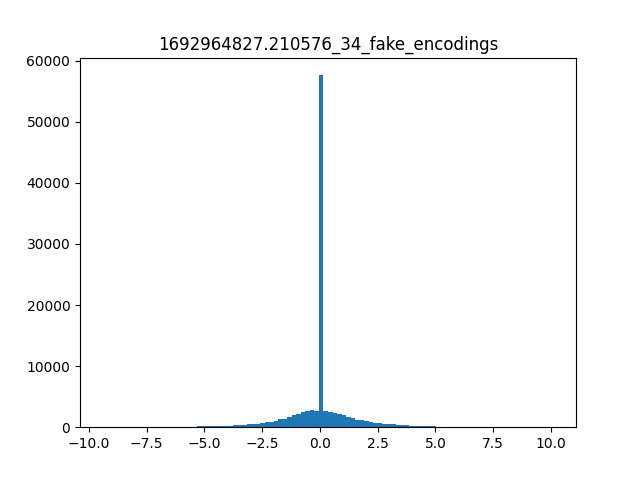
\includegraphics[width=\textwidth]{figures/4.5-results/exp9_34_hist.png}
        \caption{Histogram of the generated embeddings for Experiment 9 in epoch 34.}
        \label{fig:exp9_34_hist}
    \end{subfigure}
    \begin{subfigure}{0.4\textwidth}
        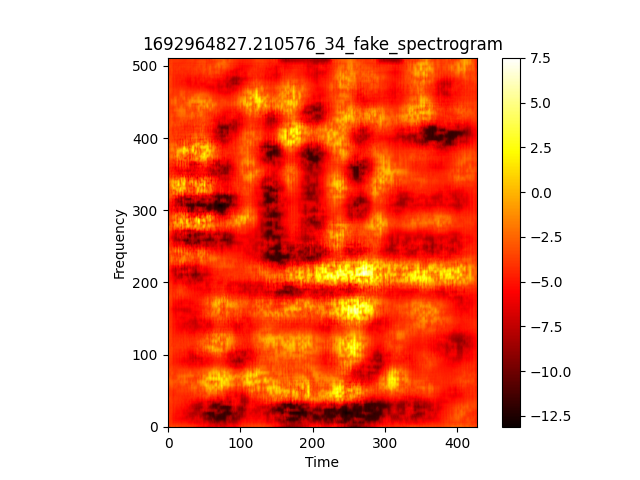
\includegraphics[width=\textwidth]{figures/4.5-results/exp9_34_spectrogram.png}
        \caption{Spectrogram generated in Experiment 9 in epoch 34.}
        \label{fig:exp9_34_spectrogram}
    \end{subfigure}
    \caption{Results of Experiment 9 in epoch 34.}
    \label{fig:exp9_34_results}
\end{figure}

\begin{figure}[!ht]
    \centering
    \begin{subfigure}{0.3\textwidth}
        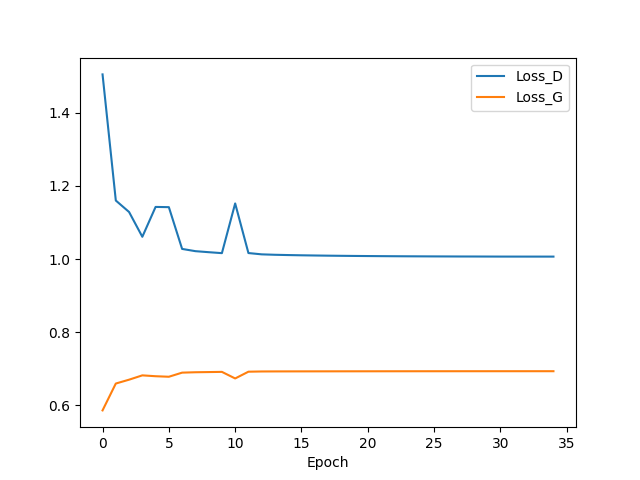
\includegraphics[width=\textwidth]{figures/4.5-results/exp9_loss.png}
        \caption{Evolving losses throughout the training process for Experiment 9.}
        \label{fig:exp9_loss}
    \end{subfigure}
    \begin{subfigure}{0.3\textwidth}
        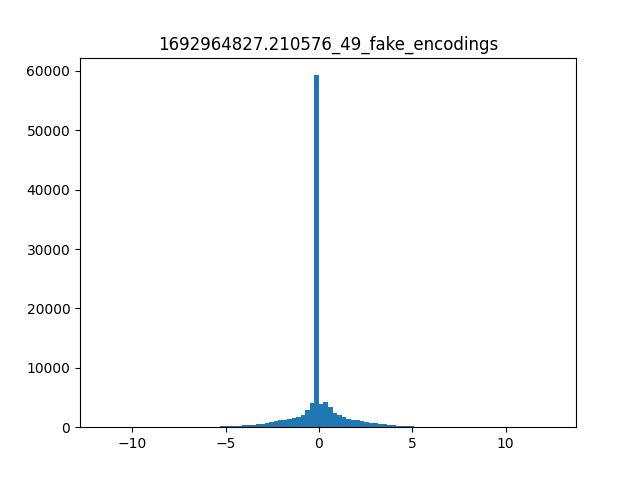
\includegraphics[width=\textwidth]{figures/4.5-results/exp9_hist.png}
        \caption{Histogram of the generated embeddings for Experiment 9.}
        \label{fig:exp9_hist}
    \end{subfigure}
    \begin{subfigure}{0.3\textwidth}
        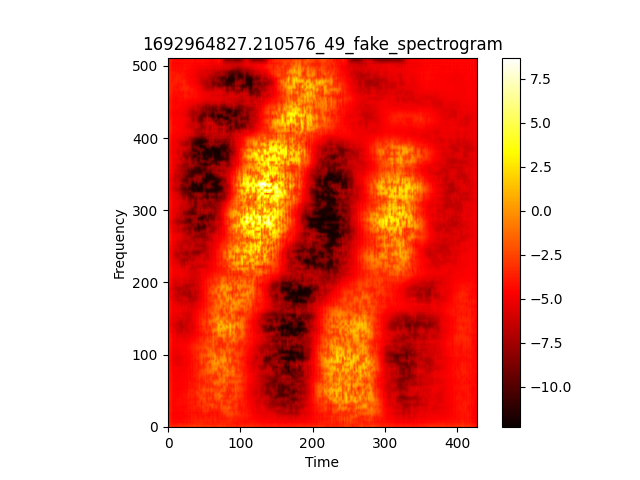
\includegraphics[width=\textwidth]{figures/4.5-results/exp9_spectrogram.png}
        \caption{Spectrogram generated in Experiment 9.}
        \label{fig:exp9_spectrogram}
    \end{subfigure}
    \caption{Results of Experiment 9 at the end of training.}
    \label{fig:exp9_results}
\end{figure}